\documentclass[a4paper]{article}

\usepackage[english]{babel}
\usepackage[margin=1in]{geometry}
\usepackage[utf8]{inputenc}
\usepackage{amsmath}
\usepackage{graphicx}
\usepackage[colorinlistoftodos]{todonotes}
\usepackage{physics} %for bra-ket notation
\usepackage{setspace} %for double spacing
\usepackage[acronym]{glossaries}

%Term definitions
\newacronym{roc}{ROC}{radius of curvature}
\newacronym{stirap}{STIRAP}{stimulated Raman adiabatic passage}
\newacronym{hbt}{HBT}{Hanbury Brown and Twiss}
\newacronym{hom}{HOM}{Hong--Ou--Mandel}

\usepackage[
backend=biber,
style=nature
]{biblatex}
\addbibresource{Humboldt-proposal.bib}
\usepackage{csquotes}

\title{Heralded Photon Storage in a Single Atom Strongly Coupled to Crossed Cavities}
\author{Joseph Christesen}
%\author{}
\date{\vspace{-5ex}}


\begin{document}
\maketitle

\onehalfspacing

\section{Introduction}

\indent\indent The union of quantum mechanics and information science has led to the birth of the field of quantum information whose study has subsequently produced a considerable number of theoretical discoveries including various quantum algorithms and communication protocols such as Shor's algorithms and BB84 as well as discoveries of advanced technological capabilities to study and control individual systems such as neutral atoms, ions, and NV-centers~\cite{Kimble2008}. In order to realize the incredible potential of these various individual quantum systems, they need to be able to communicate and transmit quantum bits, qubits, between one another through a quantum channel of a quantum network. Much like a classical network, a quantum network needs to be able to transmit data with high fidelity and efficiency between remote nodes, and for a fiber-based quantum network, losses in the fibers due to absorption cause an exponential decrease in the probability of successful transfer of qubits with distance. However, these losses can be overcome by dividing the distance between remote nodes into smaller segments and using quantum repeaters at the intersection between these segments.

Therefore, in order to create a long-distance quantum network, a quantum memory, which is a critical component of a quantum repeater, needs to be realized with both high efficiency and high fidelity. The efficiency of a quantum memory is defined as the ratio of the number of qubits retrieved from the memory versus the number of qubits sent to the memory whereas the fidelity is a measure of the similarity of states between the output and input qubits. Beyond these two key parameters, a quantum memory for use as a quantum repeater must also include a herald, an unambiguous signal for the successful storage of a qubit. Due to the previously mentioned losses of the fiber channels, any transmission between memories will be inherently probabilistic, and therefore, a herald is essential for identifying when the quantum state has been successfully stored in the quantum memory. There are several experimental frameworks which could be utilized to produce a quantum memory, and one of the most promising is trapping a neutral atom within an optical cavity because neutral atoms do not interact strongly with the environment, they can be efficiently trapped and cooled, and the optical cavity enables optical control by providing strong coupling between light and matter.  

Quantum memories based on single neutral atoms in optical cavities have already been demonstrated, and the first successful experiment was performed in 2011 by Specht et al.~\cite{Specht2011}. This quantum memory stored the polarization degree of freedom of a photonic qubit as a superposition of two hyperfine states in a $^{87}$Rb atom through absorption of the photon, which meant the fidelity of the scheme was insensitive to photon loss. Despite a good fidelity, the scheme had issues such as a lack of a herald, and low efficiencies for both storage and retrieval due to low atom-cavity coupling and the need for the precise timing between the photon arrival and a control laser pulse. Since the work by Specht et al., there have been other quantum memory schemes, and most notably is the work by Kalb et al.~\cite{Kalb2015} where the polarization of a photonic qubit was stored in the hyperfine states of a $^{87}$Rb atom through reflection of the photon off of the cavity which could then be detected as a herald for successful storage. Despite the increase in efficiency and the herald, the scheme, which required exact matching between the photonic spatial input mode and the cavity mode, suffered from reduced fidelity from non-mode-matched photons that were reflected from the cavity without ever interacting with the atom. 

Therefore, substantial improvement over previous implementations is needed in order to create a quantum memory with high fidelity, high efficiency, and a herald. In this proposal, we present a plan to use the basic ideas of the Specht et al. protocol to increase the efficiency of the scheme and include a passive herald by utilizing new mirror fabrication technology to create a radically new cavity design. We believe that the high fidelity which is insensitive to photon loss of the Specht et al. protocol provides a good starting point from which to create a high quality quantum memory.

\section{High-Cooperativity Fiber Cavities}

\indent\indent To improve the efficiency of storage and retrieval of a quantum memory system, it is necessary to increase the ratio between the atom-cavity coupling rate, $g$, and the cavity decay rate, $\kappa$, and the free-space decay rate, $\gamma$. This ratio, known as the cooperativity, can be written as~\cite{Hunger2010}


\begin{equation}
C = \frac{g ^2}{2 \kappa\gamma } = \frac{3\lambda^2}{\pi^3}\frac{\mathcal{F}}{\omega_0^2}
\end{equation}

\noindent where $\mathcal{F}$ is the cavity finesse, $\omega_0$ is the cavity mode waist, and $\lambda$ is the wavelength, and it can even be used to define the upper limit for efficiency of storage and retrieval as $C/(1+C)$. Therefore to increase the cooperativity of the cavity and the efficiency of the quantum memory, it is necessary to either increase the cavity finesse or to decrease the cavity mode waist. High-finesse cavities are already used in other cavity QED experiments, and further increases in the finesse, which is inversely proportional to the transmission of the cavity mirrors, would limit the coupling of photonic qubits into or out of the cavity.  Therefore, it is more practical to focus on decreasing the cavity mode waist, which is dependent on the length of the cavity and the \gls{roc} of the two cavity mirrors, while maintaining a high finesse. 

While current mirrors used in cavity QED experiments can be positioned within tens of microns of one another, they cannot achieve small mode waists because current techniques for producing super polished mirrors only allow for a minimum \gls{roc} of $\sim$10 mm. However, fiber-based cavities with diameters of $\sim$100 $\mu$m fabricated through a new CO$_2$ laser machining technique have been demonstrated with high finesse and mode waists that are an order of magnitude smaller than current high-finesse cavities typically used in cavity QED experiments. Another advantage is that they allow for stable coupling to single-mode fibers without the need for mode matching optics as well as direct integration of the cavity into a fiber-based quantum network~\cite{Uphoff2015a,Hunger2010}. These fiber-based cavity mirrors are fabricated using a new laser machining process where a high-power CO$_2$ laser pulse with a wavelength of 9.3 $\mu$m is focused on the end of an optical fiber and creates a smooth, concave surface through melting and evaporation due to intense local heating. The wavelength of the CO$_2$ laser was chosen because it corresponds to a maximum of the absorption of the fiber, which limits the absorption depth and the subsequent heating, melting, and evaporation to a region very near the surface. This local surface melting along with surface tension allow for the formation of the ultra-smooth concave surface as opposed to a convex surface as one might expect by melting the end of a fiber. The exact shape of the fiber end, including the curvature and eccentricity, can be controlled via the beam profile and polarization of the CO$_2$ laser pulse, which allows for precise tailoring of cavity parameters.

In order to transform these fibers into mirrors for use in a cavity, the fibers are coated with a commercial high-reflection coating using an ion beam sputtering technique to control the reflectivity and transmission of the fiber ends. These coatings are especially important because they will determine the finesse of the cavity, which needs to be comparable to current cavities used in cavity QED experiments, otherwise the gains in cooperativity could be undone by the loss in finesse. With the ion-beam sputtering technique, it is possible to create high-finesse cavities with values $\geq 1.7\times10^5$.  It is also important to make the cavity single sided such that photons only exit through one side of the cavity to allow for efficient collection of the emitted photons. Therefore, the transmission will be made different for two sides of the cavity where one side is a high reflector (3 ppm transmission) and the other is an outcoupler with about 100 times more transmission for the design wavelength.


\section{Heralded Quantum Memory Scheme}

\begin{figure}
\centering
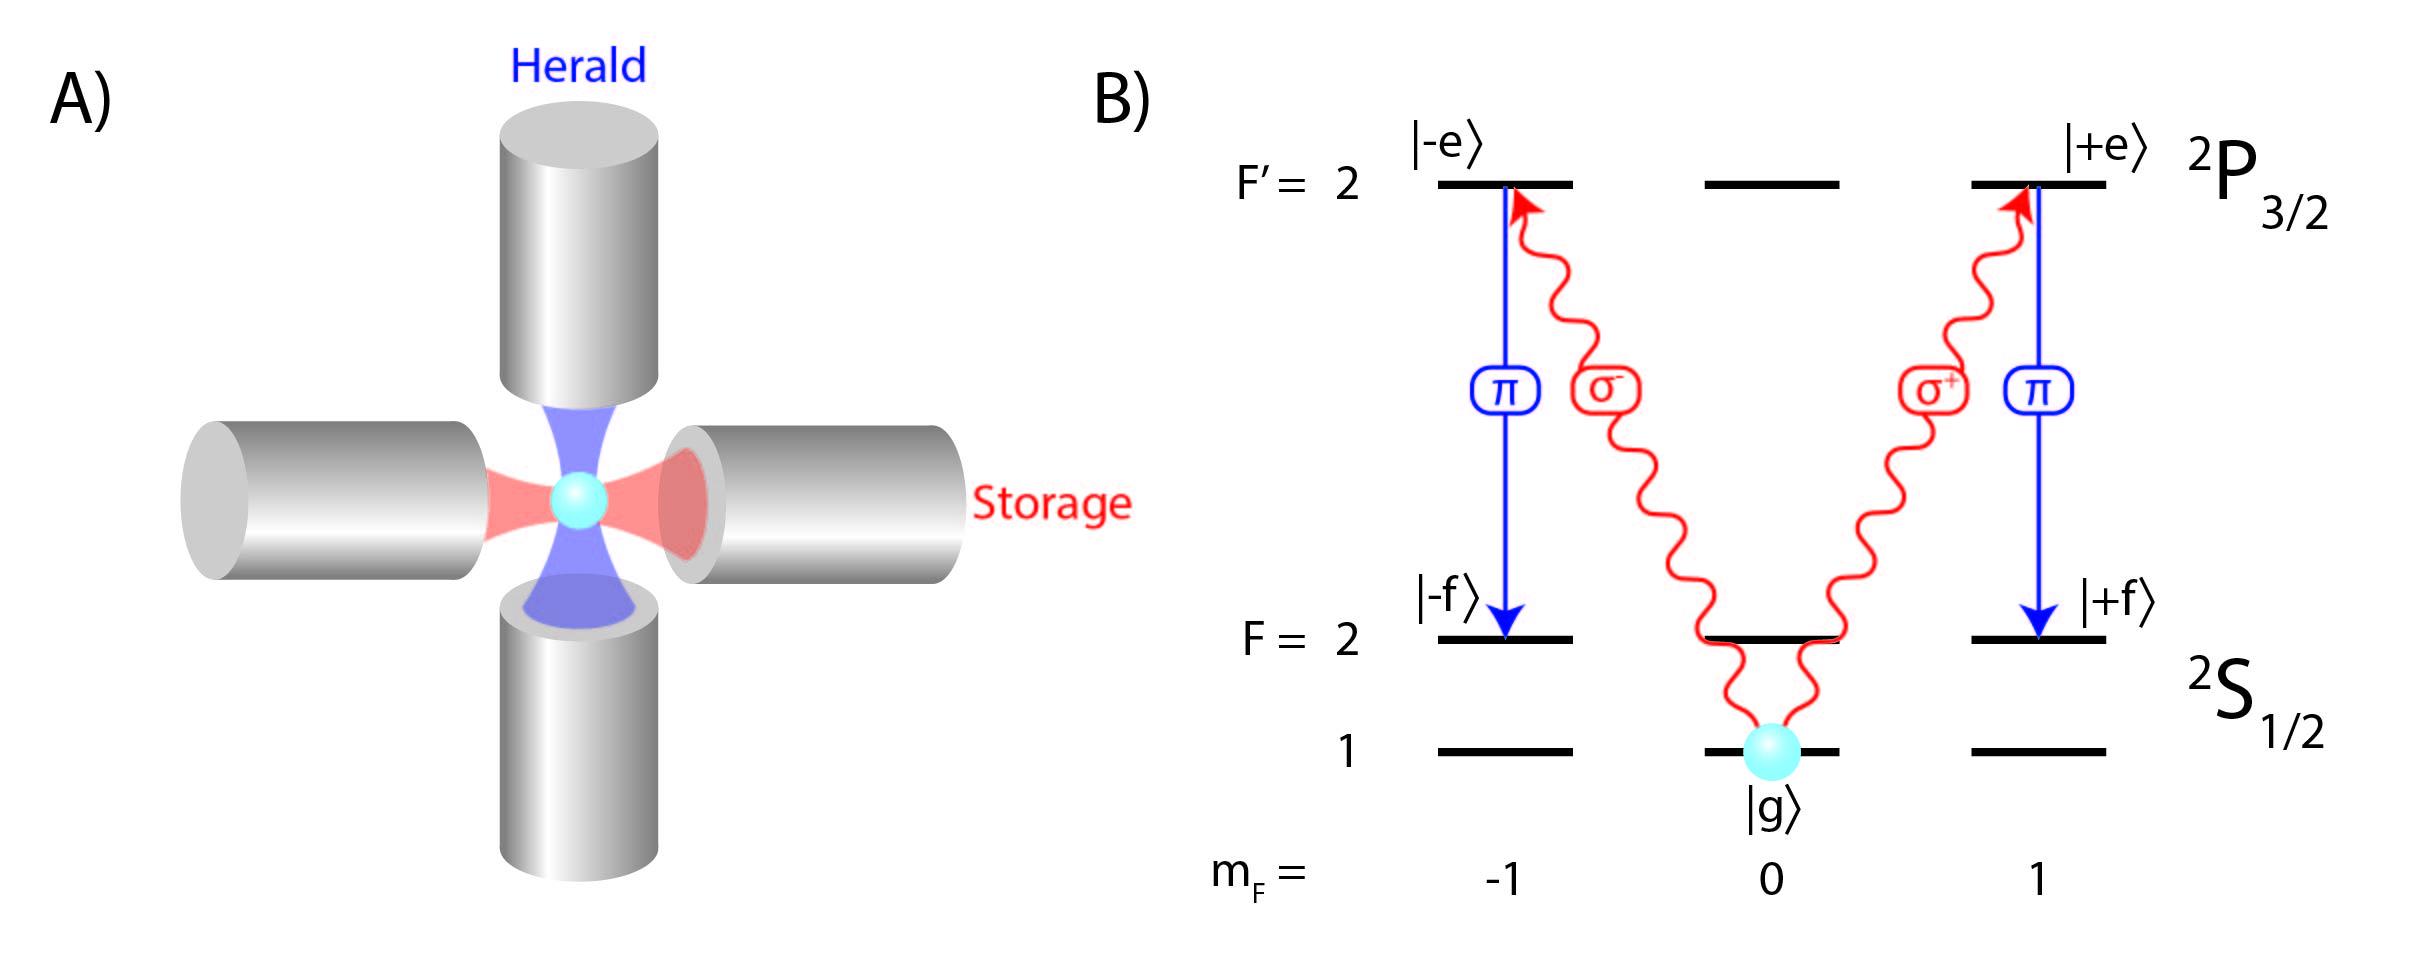
\includegraphics[width=1\textwidth]{Fig_1_Quantum_Memory_Scheme_v2-01.jpg}
\caption{\label{fig:quantumScheme} Quantum Memory Scheme. A) An illustration of the crossed cavity design with the storage cavity (left--right) and the herald cavity (up--down). B) The atomic energy levels for the quantum memory scheme in which a photon of arbitrary polarization (depicted as the superposition of $\sigma^-$ and $\sigma ^+$) is converted to an atomic superposition by the emission of a $\pi$-polarized herald photon (blue).}
\end{figure}

\indent\indent While the fiber mirrors enable higher storage and retrieval efficiencies, they do not directly solve the issues of including a herald and removing the control laser pulse from the Specht et al. protocol, but the size of the fiber mirrors allows the geometry of the cavity to be altered in order to include a second cavity perpendicular to the first without either of the two cavities occluding one another. By using two perpendicular cavities in a crossed configuration, we will be able to use one cavity for storage and retrieval and the other cavity to herald the quantum memory as illustrated in Figure~\ref{fig:quantumScheme}A. The atomic levels which will be used for the quantum memory are depicted in Figure~\ref{fig:quantumScheme}B and are the same as  those used in the previous work by Specht et al.

The  levels, which will be used for the quantum memory are the $\ket{F=1, m_F=0}$ state of the 5$^2$S$_{1/2}$ electronic level, the $\ket{F'=2, m_F=\pm 1}$ state of the 5$^2$P$_{3/2}$ electronic level, and the $\ket{F=2, m_F=\pm 1}$ state of the 5$^2$S$_{1/2}$ electronic level, which will be referred to as $\ket{g}$, $\ket{\pm e}$, and $\ket{\pm f}$, respectively. The atom is cooled and loaded into the center of the two cavities via a magneto-optical trap (MOT) and prepared in state $\ket{g}$. The photon, which is to be stored by the quantum memory, will be resonant with the D$_2$ line at 780 nm, and the qubit to be stored will be encoded as a superposition of right, $\ket{\sigma^+}$, and left, $\ket{\sigma^-}$, circularly polarized light, which can be written as $\alpha \ket{\sigma^+} + \beta \ket{\sigma^-}$ where $\alpha$ and $\beta$ are complex amplitudes. This quantum state of the polarization of the photonic qubit will be stored as a superposition of the $\ket{\pm f}$ states. However, we want to transfer the atomic state directly into $\ket{\pm f}$  instead of $\ket{\pm e}$  in order prevent spontaneous emission into another state such as  $\ket{F=2, m_F=0, \pm2}$, which would reduce the fidelity of the quantum memory. The transition from $\ket{\pm e}$ to any of the $\ket{F=2, m_F=0, \pm2}$ states is actually more favorable than the transition from $\ket{\pm e}$ to $\ket{\pm f}$ due to the transition dipole matrix element, which is why it is imperative to suppress these other transitions.

In the previous work by Specht et al., this transfer was done through a process called \gls{stirap}. \Gls{stirap} uses a control laser to off-resonantly couple states $\ket{\pm e}$ and $\ket{\pm f}$ to one another such that the population transfer occurs from $\ket{g}$ to $\ket{\pm f}$ without any transfer of state population into $\ket{\pm e}$, thereby preventing the state decay into the $\ket{F=2, m_F=0, \pm2}$ states. While the \gls{stirap} process works, it is very sensitive to the timing and shape of the incoming photon as well as the shape and intensity of the control laser. In the crossed-cavity design, the herald cavity passively couples $\ket{\pm e}$ and $\ket{\pm f}$  without the need for a \gls{stirap} process, but it needs to be engineered to prevent coupling between the $\ket{\pm e}$ and $\ket{F=2, m_F=0, \pm2}$ states.

In order for the herald cavity to only couple $\ket{\pm e}$ and $\ket{\pm f}$, the herald photon must contain no information about the photonic qubit to be stored, which means the herald cavity must couple $\ket{+e}$ and $\ket{+f}$ as well as $\ket{-e}$ and $\ket{-f}$. This is only possible through a $\pi$-polarized herald. The electric field of $\pi$-polarized light is parallel to the storage cavity axis, and it is special because it is the only polarization mode not supported by the storage cavity and contains no $\ket{\sigma^+}$ or $\ket{\sigma^-}$ components. The herald cavity, which is oriented perpendicular to the storage cavity, has a polarization eigenmodes $\pi$  and V, where V can be rewritten as $\frac{1}{\sqrt{2}}[\ket{\sigma^+}+\ket{\sigma^-}]$. Since the V polarization contains $\ket{\sigma^+}$ and $\ket{\sigma^-}$ components, the herald cavity must lift the degeneracy of these polarization eigenmodes and split the modes by several cavity line widths such that only the $\pi$-polarized mode is coupled. This can be achieved by adding an eccentricity to the fiber mirrors and creating a birefringent cavity, which has already been demonstrated by adjusting the shape and polarization of the CO$_2$ laser during the machining of the fiber mirrors~\cite{Uphoff2015a}. 

After detection of the herald, the atom is in the quantum memory state $\ket{f}$ where it is stored, and after some storage time, it is necessary to retrieve the photonic qubit from the memory. With the crossed cavity scheme, a $\pi$-polarized photon resonant with the heralding cavity is sent into the cavity, and since the storage cavity couples states $\ket{g}$ and $\ket{\pm e}$, the atom will transition from state $\ket{\pm f}$ to $\ket{g}$ emitting a photon with the same polarization as the one that was stored. In this way, the retrieval process is the exact opposite procedure as the storage process, and it can be controlled in a deterministic manner.  

\section{Experimental Setup}

\indent\indent In order to experimentally realize the quantum memory scheme described above, the first step will be to fabricate the fiber cavities, and fully characterize them by measuring various mirror and cavity parameters including the finesse, line width, and mirror losses. It is essential to know these parameters before the cavities are placed under a vacuum of 10$^{-11}$ mbar, which is to prevent any interaction between the $^{87}$Rb atom and its environment, as the high vacuum restricts any simple alterations or exchanges of fibers. Along with constructing the vacuum system and cavity setup, we will also need to control the six lasers which will be used to load, trap, cool, and study an atom in the cavities. Due to the narrow line width of the atomic transitions and the cavity, we must have precise control over the frequency, amplitude, and pulse shape of the lasers which we will achieve by locking their frequency to a frequency comb as a frequency standard, locking their power to the transmission through the cavities, and shaping the pulse by using acousto-optic modulators controlled through high speed electronics as switches.

After the experiment has been successfully constructed, the first test will be to detect falling atoms through each cavity by monitoring transmission of light through the cavities. When the falling atom enters the cavities, it will cause a splitting of the cavity modes, and a subsequent dip in transmission. While this is a basic experiment, it will demonstrate two key features of the system, namely, that atoms can be loaded into the cavities and that the cavities can detect the atoms. It will also enable fine tuning of the system components such as alignment of the fibers which is controlled by piezo positioners, the locking of the cavity, and the number of atoms entering the cavity region. After the system has been fine-tuned, we will then move on to trapping a falling atom within the cavities and cooling it to its motional ground state. This is important because the efficiency of memory is dependent on the atom being trapped in the center of cavity. While these first experiments are very basic tests of the cavities, it is important to confirm the cavities operate in a manner which is similar to that which is predicted by theory as this will be the first time that an atom will be trapped by two cavity modes from two high-cooperativity cavities.

After the cavities have been properly adjusted and an atom has been trapped in the cavities, we will start testing the memory scheme. This will involve testing the key components of the quantum memory including fidelity, efficiency, and the herald. The fidelity of the memory will be obtained by using quantum state tomography to measure the state of the photonic qubit, the efficiency will be measured by recording the number of output photonic qubits relative to the number of input qubits, and the performance of the herald will be measured as the ratio of detected herald photons relative to successful storage attempts. Although these parameters are relatively straightforward to measure, the complexity and difficulty of the quantum memory will come from optimizing experimental parameters and identifying and suppressing experimental errors in order to achieve the highest possible efficiency and fidelity for the system.

While creating a quantum memory with high efficiency, high fidelity, and a herald is the goal of this proposal, the optical fiber based crossed cavity geometry opens up a wide range of future experiments in the fields of quantum information and atomic physics including new schemes for electromagnetically induced transparency, photon-photon gates, and quantum memories at telecom wavelengths. Storing qubits at telecom wavelengths would be the next experimental step of this proposal as it brings a full scale quantum network closer to reality by eliminating the need for a frequency conversion from near IR to telecom wavelengths and allowing for repeaters to be placed further away from one another.

\section{Conclusion}

\indent\indent To enable long distance communication between individual systems over a quantum network, one must develop a quantum memory with high efficiency, high fidelity, and a herald, and while there have been several implementations of a quantum memory, none has been able to achieve all three simultaneously. In this proposal, we detail a quantum memory scheme which improves on the high fidelity scheme of Specht et al. by using a new technological development in the fabrication of optical-fiber based cavities in order to increase the storage and readout efficiency through a reduction of mode waist as well as to implement a new crossed-cavity design to enable a passive herald.  Beyond the quantum memory scheme proposed here, the large single-atom cooperativity of two perpendicular cavity modes coupled to a single atom permitted through the use optical fiber based cavity mirrors in a crossed-cavity geometry will open up a wide variety of new possibilities in quantum information as well as cavity-based atomic physics.


\printbibliography

\end{document}